\documentclass[tikz,border=10pt]{standalone}
\usepackage{tikz}
\usepackage{amsmath}

\begin{document}

%===============================
% First visualization: diagonal hyperplane
%===============================
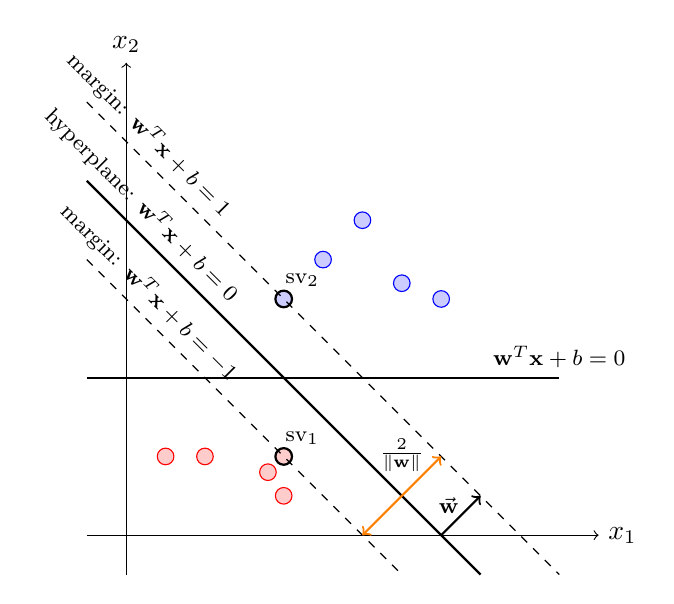
\begin{tikzpicture}[
    % Styles
    class1/.style={blue, fill=blue!20, draw=blue},   % positive class
    class2/.style={red,  fill=red!20,  draw=red},    % negative class
    supvec/.style={thick, draw=black, circle, inner sep=2pt}  % highlight support vectors
]

  % Axes
  \draw[->] (-0.5,0) -- (6,0) node[right] {$x_1$};
  \draw[->] (0,-0.5) -- (0,6) node[above] {$x_2$};

  % Class 1 (blue circles): all satisfy x1+x2 > 5 (above upper margin)
  \foreach \x/\y in {3/4, 4/3, 3.5/3.2, 2.5/3.5} {
    \draw[class1] (\x,\y) circle (3pt);
  }

  % Class 2 (red circles): all satisfy x1+x2 < 3 (below lower margin)
  \foreach \x/\y in {1/1, 2/0.5, 0.5/1, 1.8/0.8} {
    \draw[class2] (\x,\y) circle (3pt);
  }

  % Red support vector (on x1+x2=3)
  \draw[class2] (2,1) circle (3pt);
  \draw[supvec] (2,1) circle (3pt) node[above right,font=\footnotesize] {$\text{sv}_1$};
  % Blue support vector (on x1+x2=5)
  \draw[class1] (2,3) circle (3pt);
  \draw[supvec] (2,3) circle (3pt) node[above right, font=\footnotesize] {$\text{sv}_2$};

  % Decision boundary: x1 + x2 = 4
  \draw[thick]
    (-0.5,4.5) -- (4.5,-0.5)
    node[pos=0.1, above, sloped, font=\footnotesize] {hyperplane: $\mathbf{w}^T \mathbf{x} + b = 0$};

  % Margin lines: x1 + x2 = 5  and  x1 + x2 = 3
  \draw[dashed]
    (-0.5,5.5) -- (5.5,-0.5) node[pos=0.1, above, sloped, font=\footnotesize] {margin: $\mathbf{w}^T \mathbf{x} + b = 1$};
  \draw[dashed]
    (-0.5,3.5) -- (3.5,-0.5) node[pos=0.15, above, sloped,font=\footnotesize] {margin: $\mathbf{w}^T \mathbf{x} + b = -1$};

  % Normal vector w = (1,1)
  \draw[->,thick]
    (4.0,0.0) -- (4.5,0.5) node[midway,above left=-3pt,font=\footnotesize] {$\vec{\mathbf{w}}$};

  % Annotate margin width = 2/||w||
  \draw[<->, thick, orange](3.0,0.0) -- (4.0,1.0) node[midway,above=5pt, black, font=\footnotesize] {$\frac{2}{\|\mathbf{w}\|}$};

  % Decision boundary: horizontal line x_2 = 2
\draw[thick]
    (-0.5,2) -- (5.5,2)
    node[above, font=\footnotesize] {$\mathbf{w}^T \mathbf{x} + b = 0$};

\end{tikzpicture}

\end{document}
